\documentclass{article}
\usepackage{tikz}
\usepackage{pgfplots}
\pgfplotsset{compat=1.16}

\begin{document}

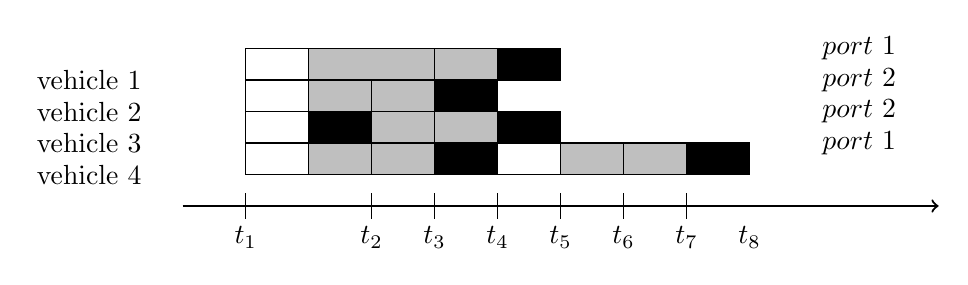
\begin{tikzpicture}[scale=0.8]
    % Draw the timeline
    \draw[->, thick] (0,0) -- (12,0);
    \foreach \x in {1,3,4,5,6,7,8} {
        \draw (\x,-0.2) -- (\x,0.2);
    }
    \node at (1,-0.5) {$t_1$};
    \node at (3,-0.5) {$t_2$};
    \node at (4,-0.5) {$t_3$};
    \node at (5,-0.5) {$t_4$};
    \node at (6,-0.5) {$t_5$};
    \node at (7,-0.5) {$t_6$};
    \node at (8,-0.5) {$t_7$};
    \node at (9,-0.5) {$t_8$};

    % Draw the vehicle labels
    \node[left] at (-0.5,2) {vehicle 1};
    \node[left] at (-0.5,1.5) {vehicle 2};
    \node[left] at (-0.5,1) {vehicle 3};
    \node[left] at (-0.5,0.5) {vehicle 4};

    % Draw the rectangles for each vehicle
    \filldraw[fill=white, draw=black] (1,2) rectangle (2,2.5);
    \filldraw[fill=gray!50, draw=black] (2,2) rectangle (4,2.5);
    \filldraw[fill=gray!50, draw=black] (4,2) rectangle (5,2.5);
    \filldraw[fill=black, draw=black] (5,2) rectangle (6,2.5);

    \filldraw[fill=white, draw=black] (1,1.5) rectangle (2,2);
    \filldraw[fill=gray!50, draw=black] (2,1.5) rectangle (3,2);
    \filldraw[fill=gray!50, draw=black] (3,1.5) rectangle (4,2);
    \filldraw[fill=black, draw=black] (4,1.5) rectangle (5,2);

    \filldraw[fill=white, draw=black] (1,1) rectangle (2,1.5);
    \filldraw[fill=black, draw=black] (2,1) rectangle (3,1.5);
    \filldraw[fill=gray!50, draw=black] (3,1) rectangle (4,1.5);
    \filldraw[fill=gray!50, draw=black] (4,1) rectangle (5,1.5);
    \filldraw[fill=black, draw=black] (5,1) rectangle (6,1.5);

    \filldraw[fill=white, draw=black] (1,0.5) rectangle (2,1);
    \filldraw[fill=gray!50, draw=black] (2,0.5) rectangle (3,1);
    \filldraw[fill=gray!50, draw=black] (3,0.5) rectangle (4,1);
    \filldraw[fill=black, draw=black] (4,0.5) rectangle (5,1);
    \filldraw[fill=white, draw=black] (5,0.5) rectangle (6,1);
    \filldraw[fill=gray!50, draw=black] (6,0.5) rectangle (7,1);
    \filldraw[fill=gray!50, draw=black] (7,0.5) rectangle (8,1);
    \filldraw[fill=black, draw=black] (8,0.5) rectangle (9,1);

    % Draw the port labels
    \node[right] at (10,2.5) {$port\ 1$};
    \node[right] at (10,2) {$port\ 2$};
    \node[right] at (10,1.5) {$port\ 2$};
    \node[right] at (10,1) {$port\ 1$};
\end{tikzpicture}

\end{document}